% Appendix D, Additional Figures (track sim, 2026-11-13). Figures are only moved here; none is redrawn.
% From the former Results: fig:const0_sd6_1anc, fig:unif1_sd6_1anc, fig:threshold_grid_sd6_1anc. From the former
% Appendix A: the other twelve. The former fig:pstar_vs_k (figures/sdim140/pstar-vs-k.pdf) is not in the build: its
% points are the qutrit points of fig:pstar_qubit_qutrit and the entries of tab:pseudo_thresholds.
% Captions say what is plotted. The numbers that the former captions quoted are in the tables of Appendix C
% (tab:kdep, tab:m0, tab:k1_depths, tab:brackets, tab:const0). The only data values left in a caption are those of
% fig:threshold_grid_sd6_2anc (check D-dip-* of jpw-review/sim/checks_appendix.py).

\section{Additional Figures}
\label{sec:additional-results}

This appendix collects the figures that \autoref{sec:results} cites and does not show. All of them come from the production runs, except the points at $p \ge p_{\mathrm{split}}$ in \autoref{fig:threshold_grid_sd6_1anc}, \autoref{fig:threshold_grid_si1000_2anc} and \autoref{fig:threshold_grid_sd6_2anc}, which come from the high-$p$ extension runs.

\subsection{One-Ancilla Layout}

\begin{figure*}[tp]
  \centering
  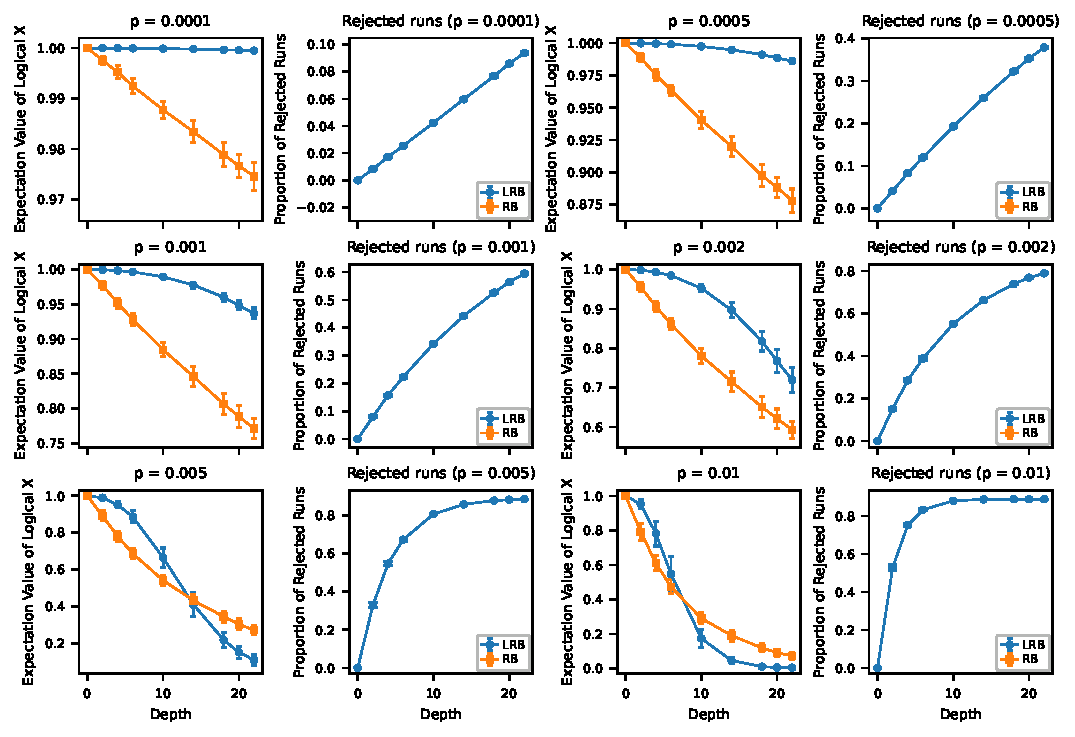
\includegraphics[width=0.78\textwidth]{figures/sdim140/sd6-1anc-const-0-nofit.pdf}
  \caption{Accepted logical signal $\langle \bar{X} \rangle$ of LRB-D (blue) and physical signal $\langle Z \rangle$ of physical RB at the same $p$ (orange) versus the depth $m$ (left panels) and fraction of rejected LRB-D shots (right panels) under terminal postselection and SD6, from the run of the one-ancilla layout. The points are joined by lines, not fits, and panels, labels, values of $p$ and error bars are as in \autoref{fig:const0_si1000_1anc}.}
  \label{fig:const0_sd6_1anc}
\end{figure*}

\begin{figure*}[tp]
  \centering
  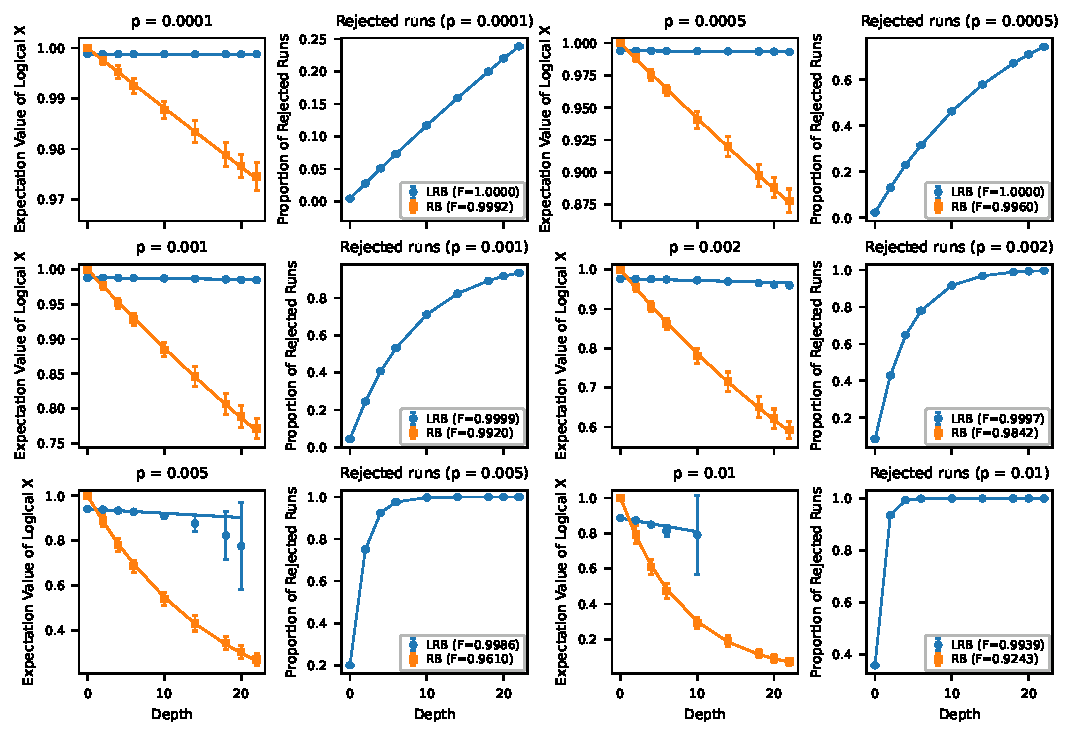
\includegraphics[width=0.78\textwidth]{figures/sdim140/sd6-1anc-unif-1-fit.pdf}
  \caption{Accepted logical signal $\langle \bar{X} \rangle$ of LRB-D (blue) and physical signal $\langle Z \rangle$ of physical RB at the same $p$ (orange) versus the depth $m$ (left panels), with the fits $F(m) = A f^m$ (lines), and fraction of rejected LRB-D shots (right panels), for uniform-interval postselection with interval $k = 1$ under SD6 in the one-ancilla layout. Panels, labels, values of $p$, legends, error bars and missing points are as in \autoref{fig:unif1_si1000_1anc}.}
  \label{fig:unif1_sd6_1anc}
\end{figure*}

\begin{figure*}[tp]
  \centering
  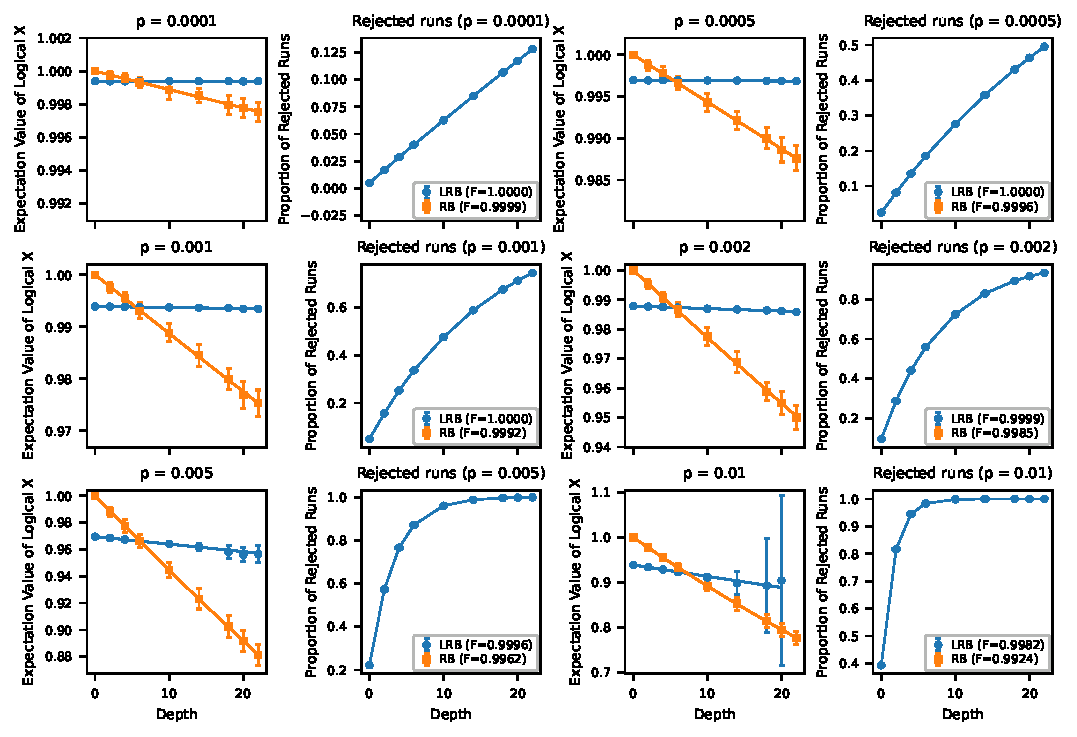
\includegraphics[width=0.78\textwidth]{figures/sdim140/si1000-1anc-unif-2-fit.pdf}
  \caption{Accepted logical signal $\langle \bar{X} \rangle$ of LRB-D (blue) and physical signal $\langle Z \rangle$ of physical RB at the same $p$ (orange) versus the depth $m$ (left panels), with the fits $F(m) = A f^m$ (lines), and fraction of rejected LRB-D shots (right panels), for uniform-interval postselection with interval $k = 2$ under SI1000 in the one-ancilla layout. Panels, labels, values of $p$, legends, error bars and missing points are as in \autoref{fig:unif1_si1000_1anc}.}
  \label{fig:unif2_si1000_1anc}
\end{figure*}

\begin{figure*}[tp]
  \centering
  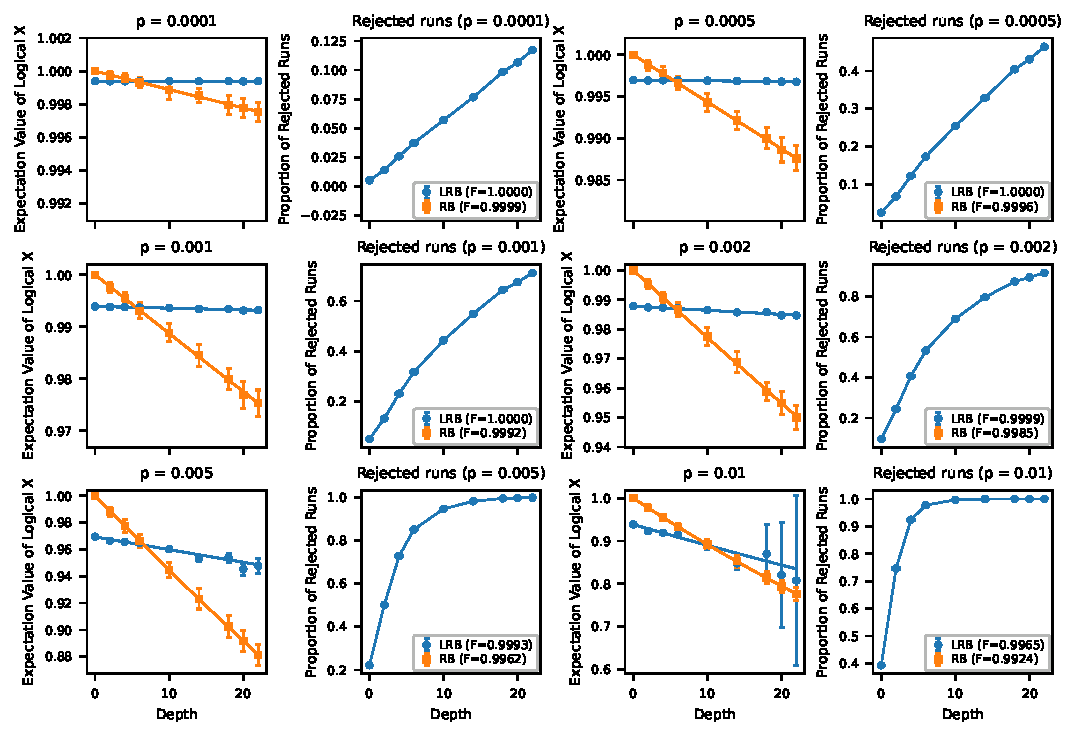
\includegraphics[width=0.78\textwidth]{figures/sdim140/si1000-1anc-unif-3-fit.pdf}
  \caption{Accepted logical signal $\langle \bar{X} \rangle$ of LRB-D (blue) and physical signal $\langle Z \rangle$ of physical RB at the same $p$ (orange) versus the depth $m$ (left panels), with the fits $F(m) = A f^m$ (lines), and fraction of rejected LRB-D shots (right panels), for uniform-interval postselection with interval $k = 3$ under SI1000 in the one-ancilla layout. Panels, labels, values of $p$, legends, error bars and missing points are as in \autoref{fig:unif1_si1000_1anc}.}
  \label{fig:unif3_si1000_1anc}
\end{figure*}

\begin{figure*}[tp]
  \centering
  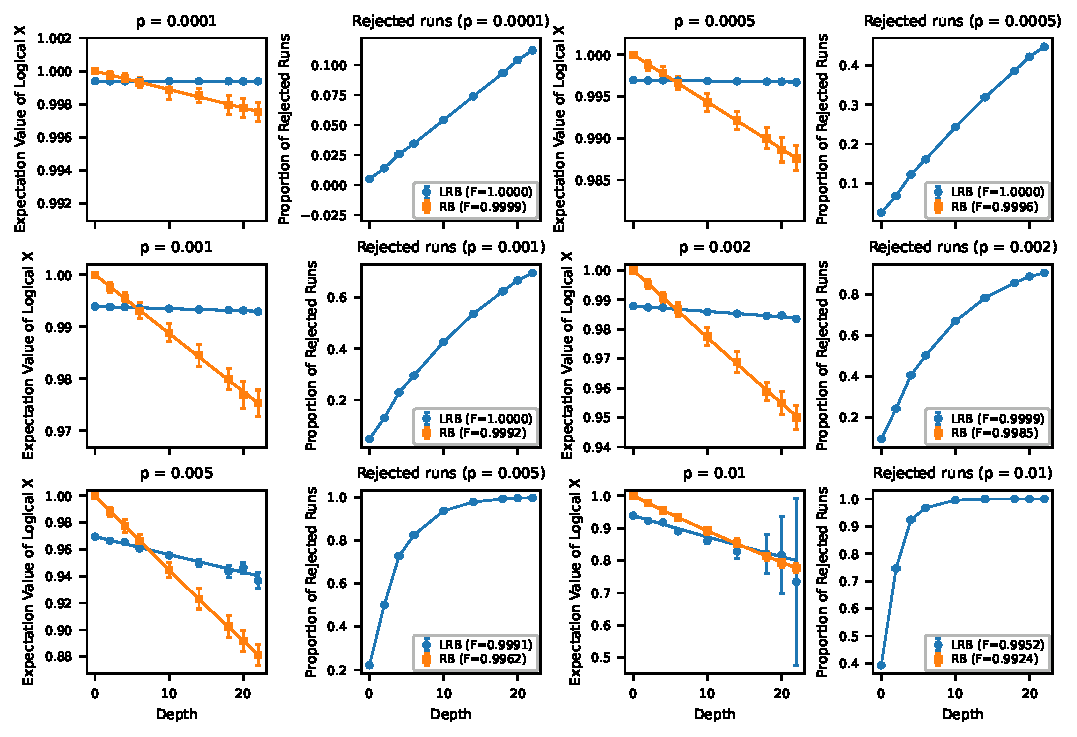
\includegraphics[width=0.78\textwidth]{figures/sdim140/si1000-1anc-unif-4-fit.pdf}
  \caption{Accepted logical signal $\langle \bar{X} \rangle$ of LRB-D (blue) and physical signal $\langle Z \rangle$ of physical RB at the same $p$ (orange) versus the depth $m$ (left panels), with the fits $F(m) = A f^m$ (lines), and fraction of rejected LRB-D shots (right panels), for uniform-interval postselection with interval $k = 4$ under SI1000 in the one-ancilla layout. Panels, labels, values of $p$, legends, error bars and missing points are as in \autoref{fig:unif1_si1000_1anc}.}
  \label{fig:unif4_si1000_1anc}
\end{figure*}

\begin{figure*}[tp]
  \centering
  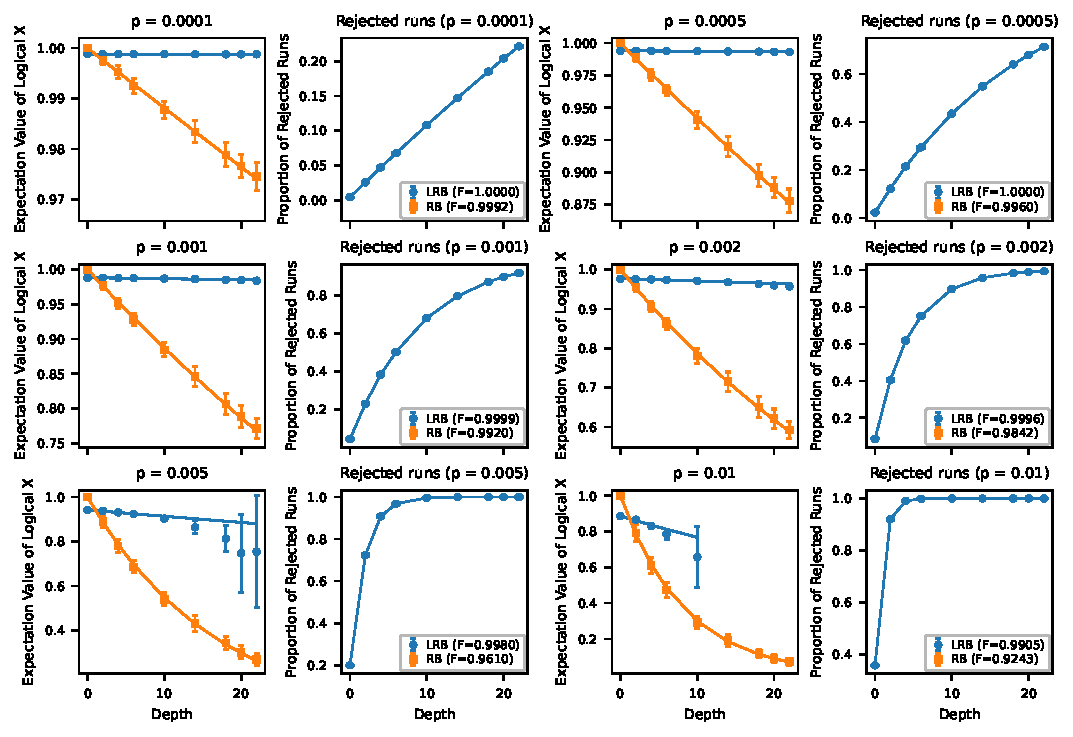
\includegraphics[width=0.78\textwidth]{figures/sdim140/sd6-1anc-unif-2-fit.pdf}
  \caption{Accepted logical signal $\langle \bar{X} \rangle$ of LRB-D (blue) and physical signal $\langle Z \rangle$ of physical RB at the same $p$ (orange) versus the depth $m$ (left panels), with the fits $F(m) = A f^m$ (lines), and fraction of rejected LRB-D shots (right panels), for uniform-interval postselection with interval $k = 2$ under SD6 in the one-ancilla layout. Panels, labels, values of $p$, legends, error bars and missing points are as in \autoref{fig:unif1_si1000_1anc}.}
  \label{fig:unif2_sd6_1anc}
\end{figure*}

\begin{figure*}[tp]
  \centering
  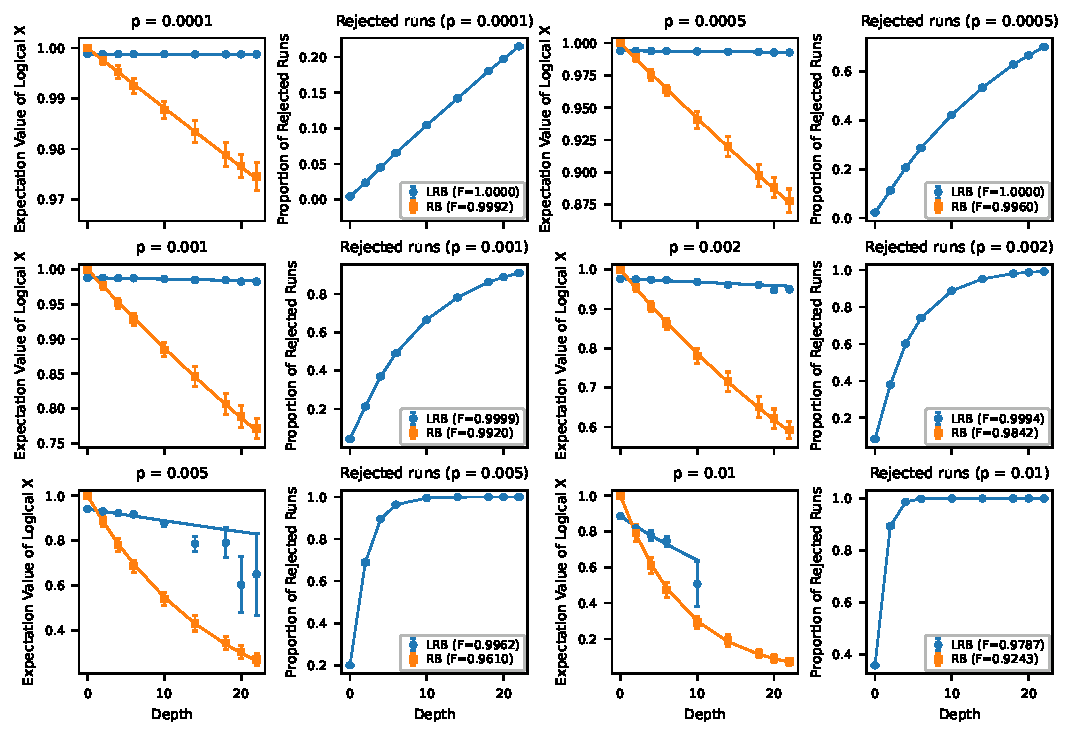
\includegraphics[width=0.78\textwidth]{figures/sdim140/sd6-1anc-unif-3-fit.pdf}
  \caption{Accepted logical signal $\langle \bar{X} \rangle$ of LRB-D (blue) and physical signal $\langle Z \rangle$ of physical RB at the same $p$ (orange) versus the depth $m$ (left panels), with the fits $F(m) = A f^m$ (lines), and fraction of rejected LRB-D shots (right panels), for uniform-interval postselection with interval $k = 3$ under SD6 in the one-ancilla layout. Panels, labels, values of $p$, legends, error bars and missing points are as in \autoref{fig:unif1_si1000_1anc}.}
  \label{fig:unif3_sd6_1anc}
\end{figure*}

\begin{figure*}[tp]
  \centering
  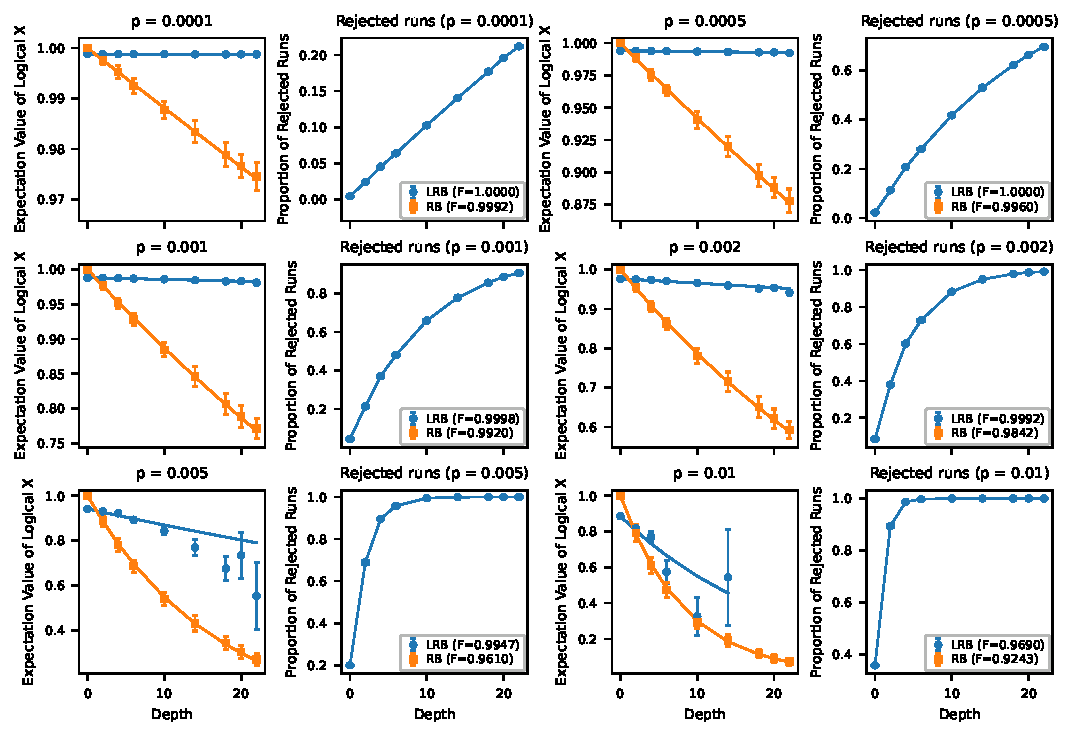
\includegraphics[width=0.78\textwidth]{figures/sdim140/sd6-1anc-unif-4-fit.pdf}
  \caption{Accepted logical signal $\langle \bar{X} \rangle$ of LRB-D (blue) and physical signal $\langle Z \rangle$ of physical RB at the same $p$ (orange) versus the depth $m$ (left panels), with the fits $F(m) = A f^m$ (lines), and fraction of rejected LRB-D shots (right panels), for uniform-interval postselection with interval $k = 4$ under SD6 in the one-ancilla layout. Panels, labels, values of $p$, legends, error bars and missing points are as in \autoref{fig:unif1_si1000_1anc}.}
  \label{fig:unif4_sd6_1anc}
\end{figure*}

\begin{figure*}[tp]
  \centering
  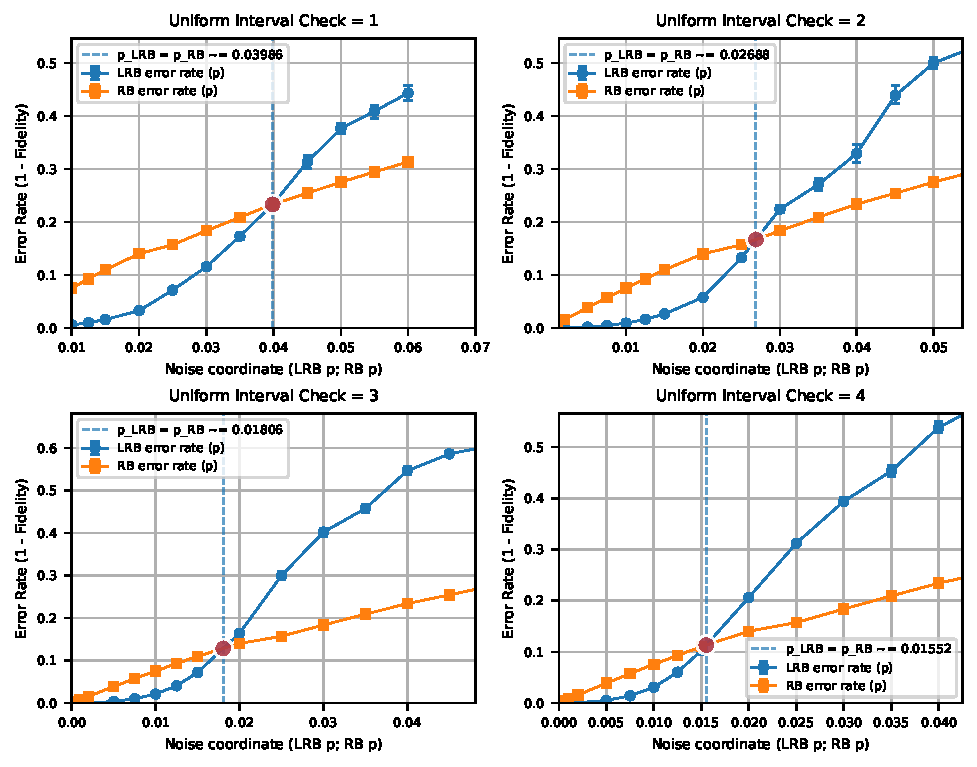
\includegraphics[width=0.75\textwidth]{figures/sdim140/sd6-1anc-threshold-grid.pdf}
  \caption{Fitted error rates per unit of depth of LRB-D (blue) and of the baseline, physical RB (orange), versus the two-qutrit gate error probability $p$ under SD6 in the one-ancilla layout, for the intervals $k = 1$ to $4$, with central 68\% intervals of the parametric bootstrap; intervals that are not visible are smaller than the markers. Each panel shows a window around $p^\star(k)$ of the grid that merges the two runs: points at $p < 0.025$ come from the production run and points at $p \ge 0.025$ from the high-$p$ extension run. Panel titles, axis labels, legends, the vertical line and the large marker are as in \autoref{fig:threshold_grid_si1000_1anc}.}
  \label{fig:threshold_grid_sd6_1anc}
\end{figure*}

\subsection{Two-Ancilla Layout}

\begin{figure*}[tp]
  \centering
  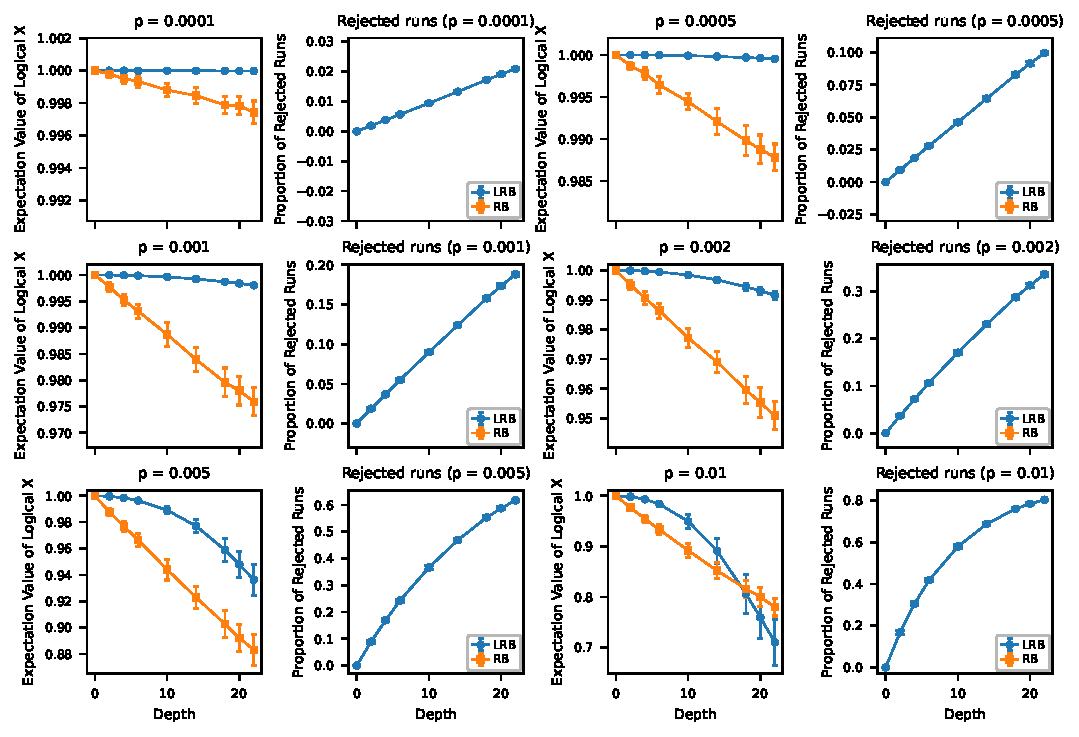
\includegraphics[width=0.78\textwidth]{figures/sdim140/si1000-conv-const-0-nofit.pdf}
  \caption{Accepted logical signal $\langle \bar{X} \rangle$ of LRB-D (blue) and physical signal $\langle Z \rangle$ of physical RB at the same $p$ (orange) versus the depth $m$ (left panels) and fraction of rejected LRB-D shots (right panels) under terminal postselection and SI1000, from the run of the two-ancilla layout. The points are joined by lines, not fits, and panels, labels, values of $p$ and error bars are as in \autoref{fig:const0_si1000_1anc}. The circuits are built as those of \autoref{fig:const0_si1000_1anc}, from 30 newly drawn sequences.}
  \label{fig:const0_si1000_2anc}
\end{figure*}

\begin{figure*}[tp]
  \centering
  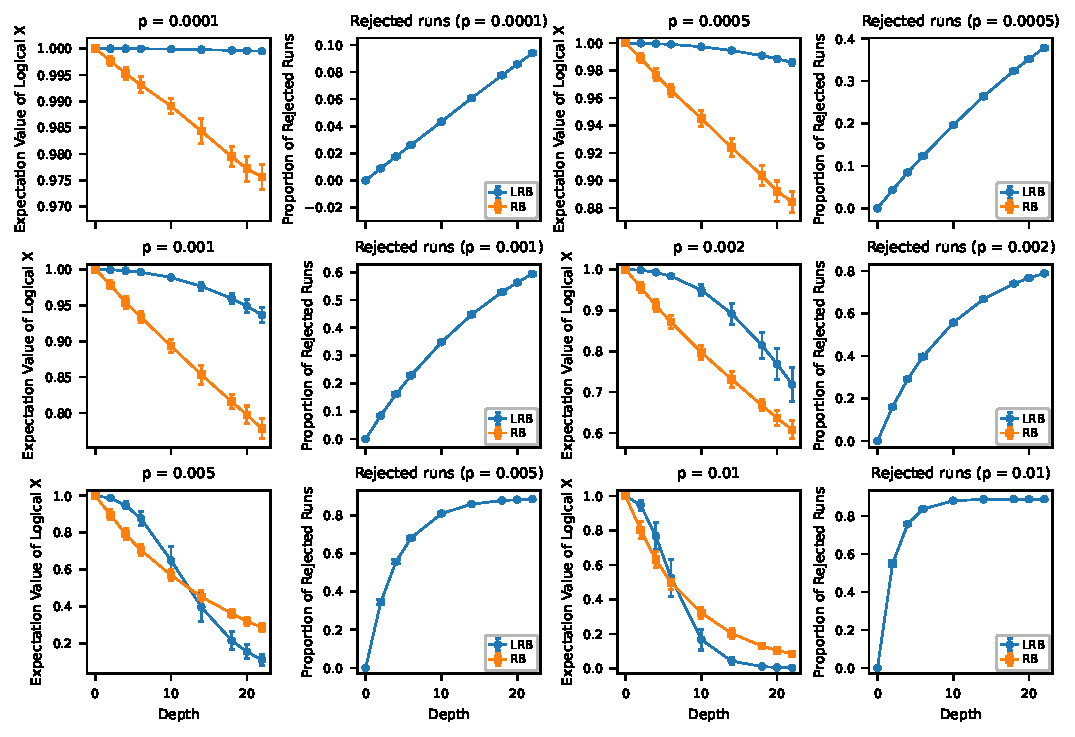
\includegraphics[width=0.78\textwidth]{figures/sdim140/sd6-conv-const-0-nofit.pdf}
  \caption{Accepted logical signal $\langle \bar{X} \rangle$ of LRB-D (blue) and physical signal $\langle Z \rangle$ of physical RB at the same $p$ (orange) versus the depth $m$ (left panels) and fraction of rejected LRB-D shots (right panels) under terminal postselection and SD6, from the run of the two-ancilla layout. The points are joined by lines, not fits, and panels, labels, values of $p$ and error bars are as in \autoref{fig:const0_si1000_1anc}. The circuits are built as those of \autoref{fig:const0_si1000_1anc}, from 30 newly drawn sequences.}
  \label{fig:const0_sd6_2anc}
\end{figure*}

\begin{figure*}[tp]
  \centering
  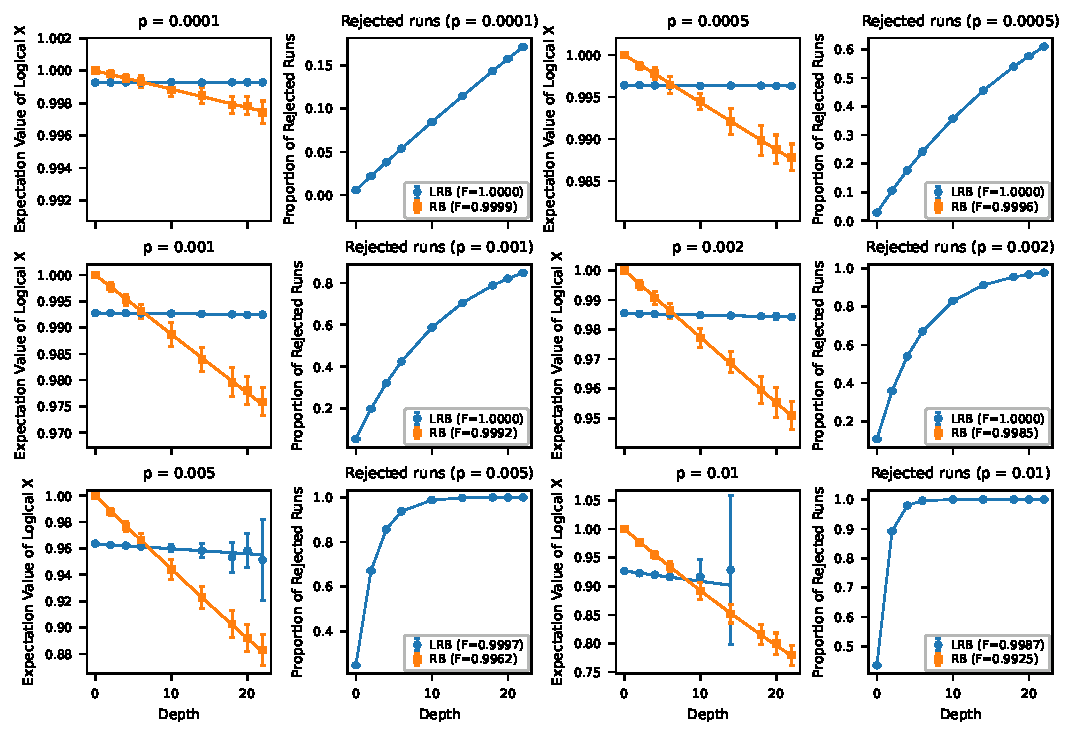
\includegraphics[width=0.78\textwidth]{figures/sdim140/si1000-conv-unif-1-fit.pdf}
  \caption{Accepted logical signal $\langle \bar{X} \rangle$ of LRB-D (blue) and physical signal $\langle Z \rangle$ of physical RB at the same $p$ (orange) versus the depth $m$ (left panels), with the fits $F(m) = A f^m$ (lines), and fraction of rejected LRB-D shots (right panels), for uniform-interval postselection with interval $k = 1$ under SI1000 in the two-ancilla layout. Panels, labels, values of $p$, legends, error bars and missing points are as in \autoref{fig:unif1_si1000_1anc}.}
  \label{fig:unif1_si1000_2anc}
\end{figure*}

\begin{figure*}[tp]
  \centering
  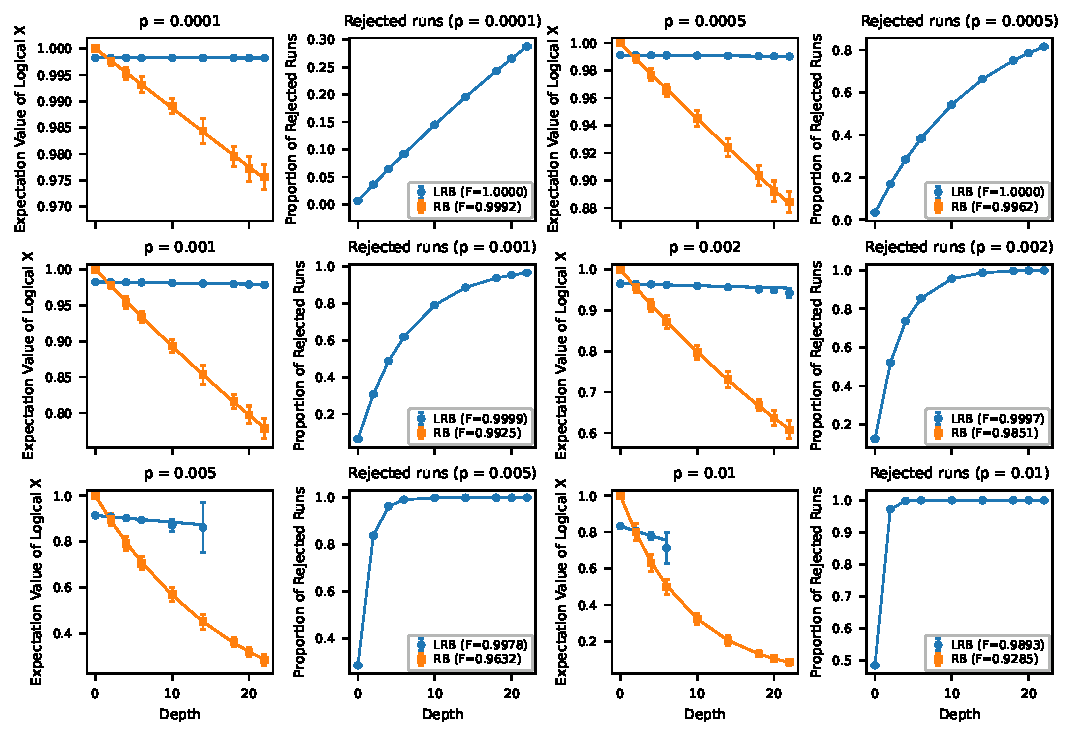
\includegraphics[width=0.78\textwidth]{figures/sdim140/sd6-conv-unif-1-fit.pdf}
  \caption{Accepted logical signal $\langle \bar{X} \rangle$ of LRB-D (blue) and physical signal $\langle Z \rangle$ of physical RB at the same $p$ (orange) versus the depth $m$ (left panels), with the fits $F(m) = A f^m$ (lines), and fraction of rejected LRB-D shots (right panels), for uniform-interval postselection with interval $k = 1$ under SD6 in the two-ancilla layout. Panels, labels, values of $p$, legends, error bars and missing points are as in \autoref{fig:unif1_si1000_1anc}.}
  \label{fig:unif1_sd6_2anc}
\end{figure*}

\begin{figure*}[tp]
  \centering
  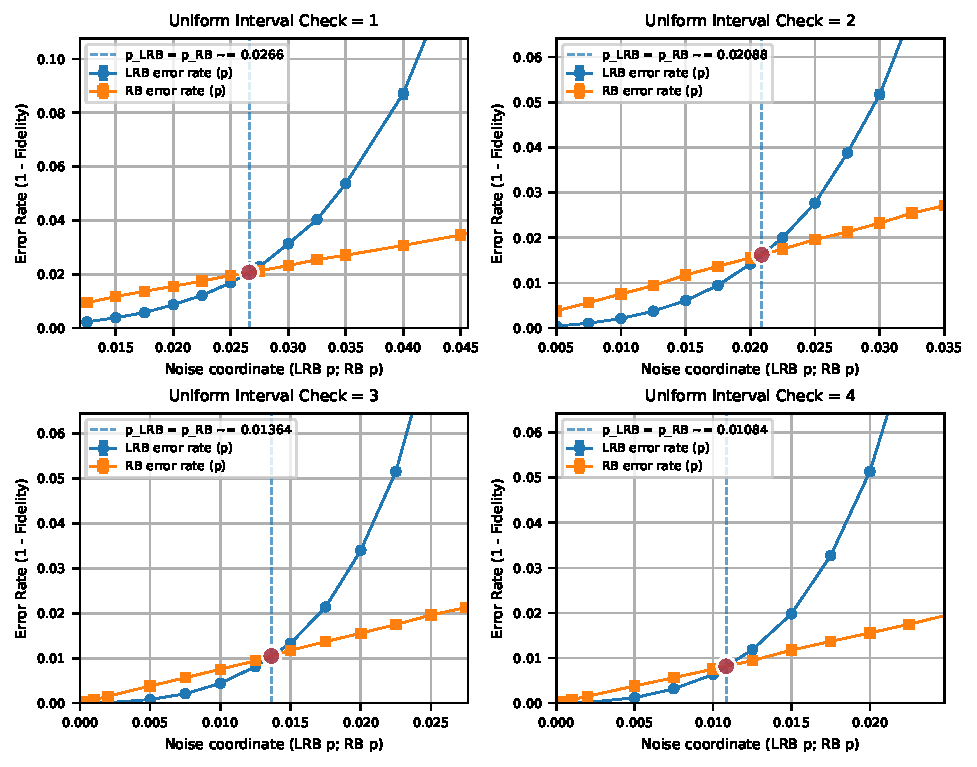
\includegraphics[width=0.85\textwidth]{figures/sdim140/si1000-conv-threshold-grid.pdf}
  \caption{Fitted error rates per unit of depth of LRB-D (blue) and of the baseline, physical RB (orange), versus the two-qutrit gate error probability $p$ under SI1000 in the two-ancilla layout, for the intervals $k = 1$ to $4$, with central 68\% intervals of the parametric bootstrap; intervals that are not visible are smaller than the markers. Each panel shows a window around $p^\star(k)$ of the grid that merges the two runs: points at $p < 0.015$ come from the production run and points at $p \ge 0.015$ from the high-$p$ extension run. Panel titles, axis labels, legends, the vertical line and the large marker are as in \autoref{fig:threshold_grid_si1000_1anc}.}
  \label{fig:threshold_grid_si1000_2anc}
\end{figure*}

\begin{figure*}[tp]
  \centering
  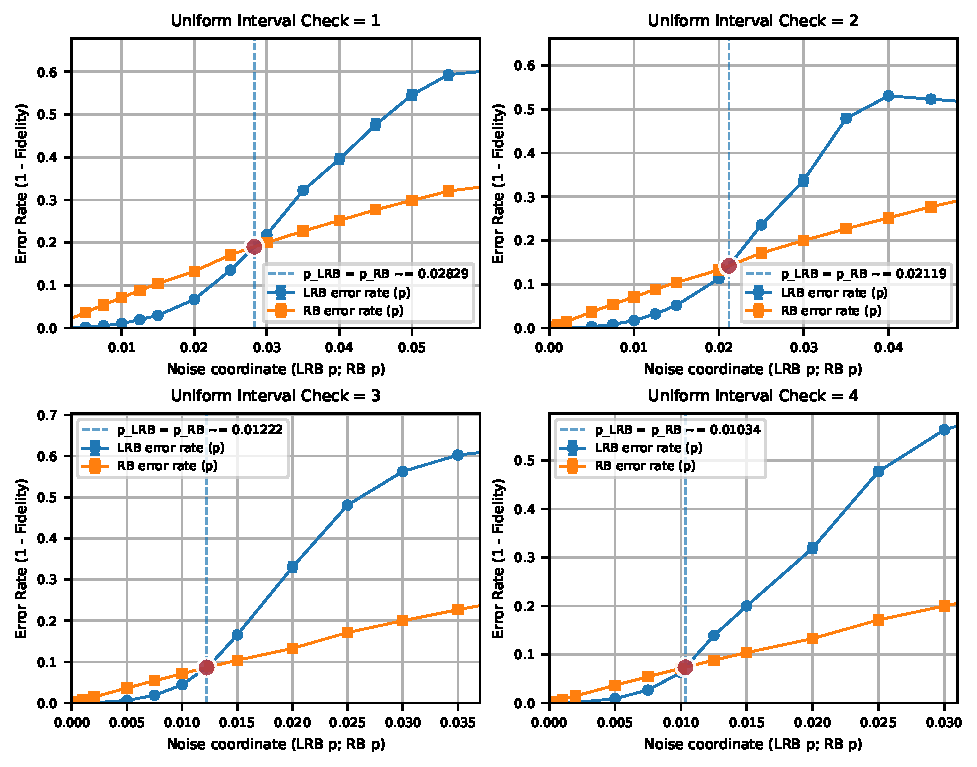
\includegraphics[width=0.80\textwidth]{figures/sdim140/sd6-conv-threshold-grid.pdf}
  \caption{Fitted error rates per unit of depth of LRB-D (blue) and of the baseline, physical RB (orange), versus the two-qutrit gate error probability $p$ under SD6 in the two-ancilla layout, for the intervals $k = 1$ to $4$, with central 68\% intervals of the parametric bootstrap; intervals that are not visible are smaller than the markers. Each panel shows a window around $p^\star(k)$ of the grid that merges the two runs: points at $p < 0.025$ come from the production run and points at $p \ge 0.025$ from the high-$p$ extension run. Panel titles, axis labels, legends, the vertical line and the large marker are as in \autoref{fig:threshold_grid_si1000_1anc}. In the $k = 2$ panel the LRB-D error rate falls from $0.531$ at $p = 0.04$ to $0.523$ at $p = 0.045$, between two fits over three depths each; the fall lies above $p^\star(2)$ and is too small to cut the grid of the search (\appref{app:campaign-search}).}
  \label{fig:threshold_grid_sd6_2anc}
\end{figure*}
